\subsection{Motivation}
\subsubsection*{Theorethischer Inhalt}
Die Workshopteilnehmer sollen zu Beginn für das Thema Affective Computing motiviert werden. Dafür gibt es einen kurze Beschreibung der Emotionen mit den Charakteristiken, wie zum Beispiel, dass Emotionen sehr schnell auftreten, aber dafür ebenfalls sehr ungenau sind \cite{emotioneninfo}. Die Intensität ist ebenfalls ein Merkmale der Emotionen. Eine hohe Intensität ist kurzzeitig und stark im Gegensatz zu einem niedrigen Intensiätsempfinden der Emotionen. Eine geringe Intensität dauert länger an und wird auch als Stimmung bezeichnet. 

\vspace{3mm}
\subsubsection*{1. Aufgabe}	
\begin{tabular}{c c}
	Zeit: 15 min & Einzelarbeit\\
\end{tabular}
\vspace{1mm}

Ziel der Aufgabe ist es, den Teilnehmern zu zeigen, dass Menschen unterschiedlich auf Ereignisse reagieren, die Emotion sowie deren Stärke kann sich stark unterschieden. Die Aufgabe soll in zwei Gruppen erfolgen, bei der die Gruppen jeweils verschiedene Webseiten angezeigt bekommen. Auf beiden Webseite sollen diese nach Informationen zu Kaffee suchen, um den via Google Formular veröffentlichten Fragebogen ausfüllen zu können. Dabei sollen die Emotionen eingetragen werden, die bei der Interaktion mit der Webseite auftreten. Während Gruppe 1 ihre Informationen in Wikipedia recherchiert \cite{kaffeewiki}, darf Gruppe 2 eine Website besuchen, welche den Inhalt grafisch ergänzt \cite{kaffecss}. \newline


\subsubsection*{Ergebnisse}
Beim durchgeführten Workshop zeigten sich die in Abbildung \ref{fig:ergebnis_1} und Abbildung \ref{fig:ergebnis_2} dargestellten Ergebnisse.

\begin{figure}[!h]
	\centering
	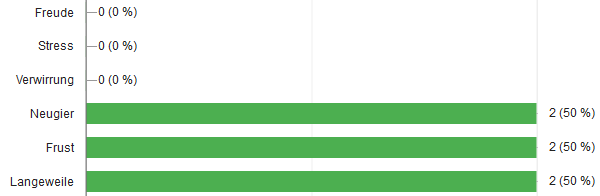
\includegraphics[width=1\linewidth]{Pictures/wiki_kaffee}
	\caption[Ergebnis der grafischen Website]{Ergebnisse der Umfrage der Gruppe mit Wikipedia}
	\label{fig:ergebnis_1}
\end{figure}

\begin{figure}[!h]
	\centering
	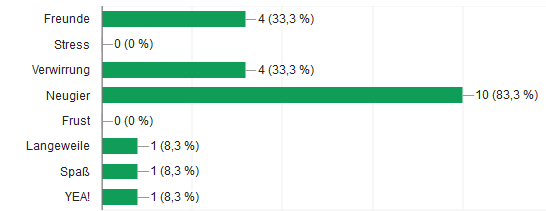
\includegraphics[width=1\linewidth]{Pictures/bizbuzz}
	\caption[Ergebnis von Wikipedia]{Ergebnisse der Umfrage der Gruppe mit Bizbrain}
	\label{fig:ergebnis_2}
\end{figure}

Die Ergebnisse zeigen auf, dass Benutzer verschieden sind und unterschiedliche Wahrnehmungen haben. Schließlich stellten wir eine möglich Erklärung dieses Verhaltens dar, indem wir den Kontext einer Person erläuterten. Der Kontext einer Person ist sehr umfangreich, wie in Abbildung \ref{fig:contextmensch} zu sehen. Als Beispiel sind hierfür der kulturelle Hintergrund, die eigenen Interessen und Hobbys sowie das soziale Umfeld zu nennen.

\begin{figure}[h!]
	\centering
	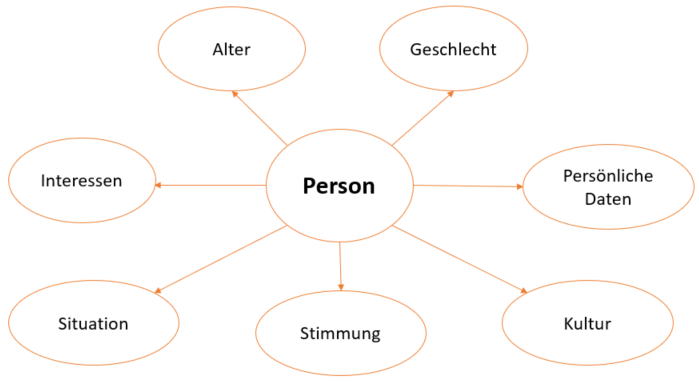
\includegraphics[width=1\linewidth]{Pictures/Context_Mensch}
	\caption[Kontext eines Menschen]{Kontext eines Menschen}
	\label{fig:contextmensch}
\end{figure}





